\subsection{The Comprehensive Summary of RAG}

Table \ref{tab:appendixb} presents a detailed analysis of the RAG studies discussed in this paper. The analysis shows that the majority of these studies have utilized external data sources to enrich the content of LLMs. A preference for multiple-hop over single-hop retrieval was noted, indicating that iterative search rounds generally yield superior results. In other words, most methods employ dense retrieval to secure higher quality candidate documents. Compared to modifying datasets in the pre-retrieval stage, more studies focus on manipulating the query to improve retrieval performance. Additionally, there is a significant emphasis on optimizing the retrieval phase, highlighting its crucial role in the research. However, there seems to be a scarcity of studies concentrating on customization in the generation stage, pointing to this as a potential area for future exploration. Overall, while the goal of RAG is to enhance the response quality of LLMs, greater efforts have been directed towards improving retrieval aspects.

\begin{table}
	\scriptsize
	\centering
	\resizebox{\linewidth}{!}{%
		\begin{tabular}{|c|c|m{5cm}|m{6cm}|} 
			\hline
			\textbf{Research} & \textbf{Year} & \textbf{Retriever} & \textbf{Generator} \\ 
			\hline
			REALM \cite{guu2020retrieval} & 2020 & BERT \cite{devlin2019bert} & Transformers \cite{vaswani2017attention} \\ 
			\hline
			kNN-LMs \cite{khandelwal2020generalization} & 2020 & FAISS \cite{8733051} & Transformers \\ 
			\hline
			RAG \cite{lewis2020retrievalaugmented} & 2020 & DPR \cite{karpukhin2020dense} & BART-Large \cite{lewis2020bart} \\ 
			\hline
			FiD \cite{izacard2021leveraging} & 2021 & BM25 \cite{robertson2009probabilistic}, DPR & T5 \cite{raffel2020exploring} \\ 
			\hline
			Webgpt \cite{nakano2021webgpt} & 2021 & Bing & GPT-3 \cite{brown2020language} \\ 
			\hline
			Re2G \cite{glass2022reg} & 2022 & BM25, DPR & BART \\ 
			\hline
			RETRO \cite{borgeaud2022improving} & 2022 & BERT & Transformer \\ 
			\hline
			DSP \cite{khattab2022demonstratesearchpredict} & 2022 & ColBERTv2 \cite{khattab2020colbert} & GPT-3.5 (text-davinci-002) \\ 
			\hline
			CoK \cite{li2024chainofknowledge} & 2023 & LLaMA2-7B \cite{touvron2023llama}, ChatGPT (gpt-3.5-turbo-0613) & ChatGPT (gpt-3.5-turbo-0613) \\ 
			\hline
			IRCOT \cite{trivedi2023interleaving} & 2023 & BM25 & GPT-3 (code-davinci-002), Flan-T5~\cite{chung2022scaling} \\ 
			\hline
			ITRG \cite{feng2024retrievalgeneration} & 2023 & Atlas \cite{ma2023query} & LLaMA-33B \\ 
			\hline
			PKG \cite{luo2023augmented} & 2023 & LLaMA-7B & InstructGPT-3.5 (text-davinic-002) \cite{ouyang2022training} \\ 
			\hline
			RA-DIT \cite{lin2024radit} & 2023 & DRAGON+ \cite{lin2023train} & LLaMA \\ 
			\hline
			Self-RAG \cite{asai2024selfrag} & 2023 & Contriever \cite{izacard2022unsupervised} & LLaMA2 (7B and 13B) , GPT-4 \cite{achiam2023gpt} \\ 
			\hline
			SURGE \cite{kang2023knowledge} & 2023 & Graph Neural Networks (GNN) \cite{hamilton2020graph} & Transformers \\ 
			\hline
			FiD-TF \cite{berchansky2023optimizing} & 2023 & BM25, SBERT \cite{reimers2019sentencebert} & T5 \\ 
			\hline
			PRCA \cite{yang2023prca} & 2023 & BM25, DPR, Contriver, SimCSE \cite{gao2021simcse}, SBERT & T5, Phoenix-7B \cite{chen2023phoenix}, Vicuna-7B \cite{vicuna2023}, ChatGLM \cite{du2022glm}, GPT-3.5 \\ 
			\hline
			REPLUG \cite{shi2023replug} & 2023 & Contriever & GPT-3 \\ 
			\hline
			AAR \cite{yu2023augmentationadapted} & 2023 & ANCE \cite{xiong2021approximate}, Contriever & Flan-T5, InstructGPT \\ 
			\hline
			Query2doc \cite{wang2023querydoc} & 2023 & BM25, DPR & GPT-3 (text-davinci-003) \\ 
			\hline
			Step-Back \cite{zheng2024take} & 2023 & PaLM-2L \cite{chowdhery2023palm} & PaLM-2L, GPT-4 \\ 
			\hline
			ITER-RETGEN \cite{shao2023enhancing} & 2023 & Contriever & InstructGPT (text-davinci-003), LLaMA2 \\ 
			\hline
			RECITE \cite{sun2023recitationaugmented} & 2023 & & PaLM, UL2 \cite{tay2023ul}, OPT \cite{zhang2022opt}, Codex \cite{chen2021evaluating} \\ 
			\hline
			PROMPTAGATOR \cite{dai2023promptagator} & 2023 & T5 & FLAN \\ 
			\hline
			UPRISE \cite{cheng2023uprise} & 2023 & GPT-Neo-2.7B \cite{black2022gptneoxb} & BLOOM-7.1B \cite{workshop2022bloom}, OPT-66B, GPT-3-175B \\ 
			\hline
			GENREAD \cite{yu2023generate} & 2023 &  & InstructGPT \\ 
			\hline
			LAPDOG \cite{huang2023learning} & 2023 & Contriever & T5 \\
			\hline
			KnowledGPT \cite{wang2023knowledgpt} & 2023 &  & GPT-4 \\ 
			\hline
			Selfmem \cite{cheng2023lift} & 2023 & BM25 & XGLM \cite{lin2022fewshot}, XLM-Rbase \cite{conneau2020unsupervised} \\ 
			\hline
			MEMWALKER \cite{chen2023walking} & 2023 & LLaMA2 & LLaMA2 \\ 
			\hline
			RECOMP \cite{xu2024recomp} & 2023 & BM25 & T5-Large \\ 
			\hline
			Rewrite-Retrieve-Read \cite{ma2023query} & 2023 & Bing & T5-Large, ChatGPT(gpt-3.5-turbo), Vicuna-13B \\ 
			\hline
			Atlas \cite{ma2023query} & 2023 & Contriever & T5 \\ 
			\hline
			DKS-RAC \cite{huang2023retrieval} & 2023 & DPR & BART \\ 
			\hline
			In-Context RALM \cite{ram2023incontext} & 2023 & BM25, BERT-base, Contriever, Spider \cite{ram2022learning} & GPT-2, GPT-Neo, GPT-J \cite{gao2021pile}, OPT, and LLaMA \\ 
			\hline
			Fid-light \cite{hofstätter2023fidlight} & 2023 & GTR-Base \cite{ni2022large} & T5 \\ 
			\hline
			FLARE \cite{jiang2023active} & 2023 & BM25, Bing & GPT-3.5 (text-davinci-003) \\
			\hline
			Chameleon \cite{jiang2023chameleon} & 2023 & ChamVS \cite{jiang2023chameleon} & ChamLM \cite{jiang2023chameleon} \\
			\hline
			ERAGent \cite{shi2024eragent} & 2024 & Bing & GPT-3.5, Falcon 1B \cite{penedo2023refinedweb} \\
			\hline
			PipeRAG \cite{jiang2024piperag} & 2024 & SBERT & RETRO \cite{borgeaud2022improving} \\
			\hline
			GenRT \cite{xu2024listaware} & 2024 & LambdaMart \cite{ai2018learning} &  \\
			\hline
			PersonaRAG \cite{zerhoudi2024personarag} & 2024 & BM25 & GPT-3.5\\
			\hline
			CRAG \cite{yan2024corrective} & 2024 & Contriever &  LLaMA2\\
			\hline
			IMRAG \cite{yang2024imrag} & 2024 & DPR & Vicuna-7B  \\
			\hline
			AiSAQ \cite{tatsuno2024aisaq} & 2024 & DiskANN \cite{pan2023lmdiskann} &  \\
			\hline
			ROPG \cite{salemi2024optimization} & 2024 & BM25, Contriever & FlanT5-XXL \\
			\hline
			RQ-RAG \cite{chan2024rqrag} & 2024 & DuckDuckGo\footnote{https://duckduckgo.com} & LLaMA2-7B \\
			\hline
			PlanRAG \cite{lee2024planrag} & 2024 & GPT-4 & GPT-4 \\
			\hline
			RARG \cite{yue2024evidencedriven} & 2024 & BM25, E5 \cite{wang2022text}& LLaMA2-7B  \\
			\hline 
			DRAGIN \cite{su2024dragin} & 2024 & BM25, SGPT \cite{muennighoff2022sgpt} & LLaMA2 (7B and 13B), Vicuna-13B  \\
			\hline
			LRUS-CoverTree \cite{ma2024reconsidering} & 2024 & k-MIPS & \\
			\hline
		\end{tabular}
	}
	\caption{The summary of Retrievers and Generators. The retrieval models and pre-trained language models explicitly mentioned in these studies have been recorded.}
	\label{tab:regencomp}
\end{table}

\begin{table}
	\centering
	\resizebox{\linewidth}{!}{
	\begin{tabular}{cccccccccc}
		\toprule
		\multirow{3}{*}{\bf Corpus} & \multirow{3}{*}{\bf Retriever} & \multicolumn{5}{c}{\bf \textsc{Mirage} Benchmark Dataset} & \multirow{3}{*}{\bf Average} \\ 
		\cmidrule(lr){3-7}
		&  & \bf MMLU-Med & \bf MedQA-US & \bf MedMCQA & \bf PubMedQA* & \bf BioASQ-Y/N &  \\
		\midrule
		None & None & 72.91 \textcolor{gray}{\scriptsize $\pm$ 1.35} & 65.04 \textcolor{gray}{\scriptsize $\pm$ 1.34} & 55.25 \textcolor{gray}{\scriptsize $\pm$ 0.77} & 36.00 \textcolor{gray}{\scriptsize $\pm$ 2.15} & 74.27 \textcolor{gray}{\scriptsize $\pm$ 1.76} & 60.69 \\
		\midrule
		\multirow{6}{*}{\makecell{\textbf{PubMed}\\ (23.9M)}} 
		& BM25 & \cellcolor{red!40.4!} 72.27 \textcolor{gray}{\scriptsize $\pm$ 1.36} & \cellcolor{red!67.5!} 63.71 \textcolor{gray}{\scriptsize $\pm$ 1.35} & \cellcolor{green!6.8!} 55.49 \textcolor{gray}{\scriptsize $\pm$ 0.77} & \cellcolor{green!73.2!} 66.20 \textcolor{gray}{\scriptsize $\pm$ 2.12} & \cellcolor{green!71.1!} 88.51 \textcolor{gray}{\scriptsize $\pm$ 1.28} & \cellcolor{green!62.8!} 69.23 \\
		& Contriever & \cellcolor{red!74.1!} 71.72 \textcolor{gray}{\scriptsize $\pm$ 1.36} & \cellcolor{red!55.5!} 63.94 \textcolor{gray}{\scriptsize $\pm$ 1.35} & \cellcolor{red!30.1!} 54.29 \textcolor{gray}{\scriptsize $\pm$ 0.77} & \cellcolor{green!71.7!} 65.60 \textcolor{gray}{\scriptsize $\pm$ 2.12} & \cellcolor{green!55.7!} 85.44 \textcolor{gray}{\scriptsize $\pm$ 1.42} & \cellcolor{green!55.2!} 68.20 \\
		& SPECTER & \cellcolor{green!5.5!} 73.19 \textcolor{gray}{\scriptsize $\pm$ 1.34} & \cellcolor{green!5.2!} 65.20 \textcolor{gray}{\scriptsize $\pm$ 1.34} & \cellcolor{red!66.8!} 53.12 \textcolor{gray}{\scriptsize $\pm$ 0.77} & \cellcolor{green!45.6!} 54.80 \textcolor{gray}{\scriptsize $\pm$ 2.23} & \cellcolor{green!7.3!} 75.73 \textcolor{gray}{\scriptsize $\pm$ 1.72} & \cellcolor{green!27.3!} 64.41 \\
		& MedCPT & \cellcolor{green!3.5!} 73.09 \textcolor{gray}{\scriptsize $\pm$ 1.34} & \cellcolor{green!54.0!} 66.69 \textcolor{gray}{\scriptsize $\pm$ 1.32} & \cellcolor{red!9.8!} 54.94 \textcolor{gray}{\scriptsize $\pm$ 0.77} & \cellcolor{green!73.7!} 66.40 \textcolor{gray}{\scriptsize $\pm$ 2.11} & \cellcolor{green!57.3!} 85.76 \textcolor{gray}{\scriptsize $\pm$ 1.41} & \cellcolor{green!63.8!} 69.38 \\
		& RRF-2 & \cellcolor{green!56.3!} 75.57 \textcolor{gray}{\scriptsize $\pm$ 1.30} & \cellcolor{red!35.6!} 64.34 \textcolor{gray}{\scriptsize $\pm$ 1.34} & \cellcolor{green!2.7!} 55.34 \textcolor{gray}{\scriptsize $\pm$ 0.77} & \cellcolor{green!80.0!} 69.00 \textcolor{gray}{\scriptsize $\pm$ 2.07} & \cellcolor{green!63.8!} 87.06 \textcolor{gray}{\scriptsize $\pm$ 1.35} & \cellcolor{green!70.3!} 70.26 \\
		& RRF-4 & \cellcolor{green!9.4!} 73.37 \textcolor{gray}{\scriptsize $\pm$ 1.34} & \cellcolor{red!15.7!} 64.73 \textcolor{gray}{\scriptsize $\pm$ 1.34} & \cellcolor{red!15.8!} 54.75 \textcolor{gray}{\scriptsize $\pm$ 0.77} & \cellcolor{green!75.6!} 67.20 \textcolor{gray}{\scriptsize $\pm$ 2.10} & \cellcolor{green!71.1!} 88.51 \textcolor{gray}{\scriptsize $\pm$ 1.28} & \cellcolor{green!66.3!} 69.71 \\
		\midrule
		
		\multirow{6}{*}{\makecell{\textbf{Wikipedia}\\(29.9M)}} 
		& BM25 & \cellcolor{green!9.4!} 73.37 \textcolor{gray}{\scriptsize $\pm$ 1.34} & \cellcolor{red!79.4!} 63.47 \textcolor{gray}{\scriptsize $\pm$ 1.35} & \cellcolor{red!36.1!} 54.10 \textcolor{gray}{\scriptsize $\pm$ 0.77} & \cellcolor{red!55.6!} 26.40 \textcolor{gray}{\scriptsize $\pm$ 1.97} & \cellcolor{red!12.4!} 71.36 \textcolor{gray}{\scriptsize $\pm$ 1.82} & \cellcolor{red!37.8!} 57.74 \\
		& Contriever & \cellcolor{green!25.0!} 74.10 \textcolor{gray}{\scriptsize $\pm$ 1.33} & \cellcolor{green!30.9!} 65.99 \textcolor{gray}{\scriptsize $\pm$ 1.33} & \cellcolor{red!38.3!} 54.03 \textcolor{gray}{\scriptsize $\pm$ 0.77} & \cellcolor{red!55.6!} 26.40 \textcolor{gray}{\scriptsize $\pm$ 1.97} & \cellcolor{red!18.6!} 69.90 \textcolor{gray}{\scriptsize $\pm$ 1.85} & \cellcolor{red!33.4!} 58.08 \\
		& SPECTER & \cellcolor{red!46.0!} 72.18 \textcolor{gray}{\scriptsize $\pm$ 1.36} & \cellcolor{red!71.4!} 63.63 \textcolor{gray}{\scriptsize $\pm$ 1.35} & \cellcolor{red!79.6!} 52.71 \textcolor{gray}{\scriptsize $\pm$ 0.77} & \cellcolor{red!79.9!} 22.20 \textcolor{gray}{\scriptsize $\pm$ 1.86} & \cellcolor{red!31.7!} 66.83 \textcolor{gray}{\scriptsize $\pm$ 1.89} & \cellcolor{red!66.3!} 55.51 \\
		& MedCPT & \cellcolor{red!57.2!} 71.99 \textcolor{gray}{\scriptsize $\pm$ 1.36} & \cellcolor{green!2.7!} 65.12 \textcolor{gray}{\scriptsize $\pm$ 1.34} & \cellcolor{red!3.1!} 55.15 \textcolor{gray}{\scriptsize $\pm$ 0.77} & \cellcolor{red!40.6!} 29.00 \textcolor{gray}{\scriptsize $\pm$ 2.03} & \cellcolor{red!3.4!} 73.46 \textcolor{gray}{\scriptsize $\pm$ 1.78} & \cellcolor{red!22.3!} 58.95 \\
		& RRF-2 & \cellcolor{green!26.9!} 74.20 \textcolor{gray}{\scriptsize $\pm$ 1.33} & \cellcolor{red!23.7!} 64.57 \textcolor{gray}{\scriptsize $\pm$ 1.34} & \cellcolor{red!16.6!} 54.72 \textcolor{gray}{\scriptsize $\pm$ 0.77} & \cellcolor{red!29.0!} 31.00 \textcolor{gray}{\scriptsize $\pm$ 2.07} & \cellcolor{green!9.7!} 76.21 \textcolor{gray}{\scriptsize $\pm$ 1.71} & \cellcolor{red!7.0!} 60.14 \\
		& RRF-4 & \cellcolor{green!5.5!} 73.19 \textcolor{gray}{\scriptsize $\pm$ 1.34} & \cellcolor{red!3.8!} 64.96 \textcolor{gray}{\scriptsize $\pm$ 1.34} & \cellcolor{red!22.6!} 54.53 \textcolor{gray}{\scriptsize $\pm$ 0.77} & \cellcolor{red!29.0!} 31.00 \textcolor{gray}{\scriptsize $\pm$ 2.07} & \cellcolor{red!9.6!} 72.01 \textcolor{gray}{\scriptsize $\pm$ 1.81} & \cellcolor{red!19.9!} 59.14 \\
		
		\bottomrule
	\end{tabular}
	}
	\caption{Part results of Accuracy (\%) of GPT-3.5 across different corpora and retrievers on Mirage. Red and green highlight \colorbox{red!50}{declines} and \colorbox{green!50}{improvements} compared to CoT (first row), with shading intensity reflecting the degree of change. Data sourced from Mirage \cite{xiong2024benchmarking}.}
	\label{tab:retrievalcomp}
\end{table}

\begin{figure}
	\centering
	\begin{subfigure}[b]{0.45\linewidth}
		\centering
		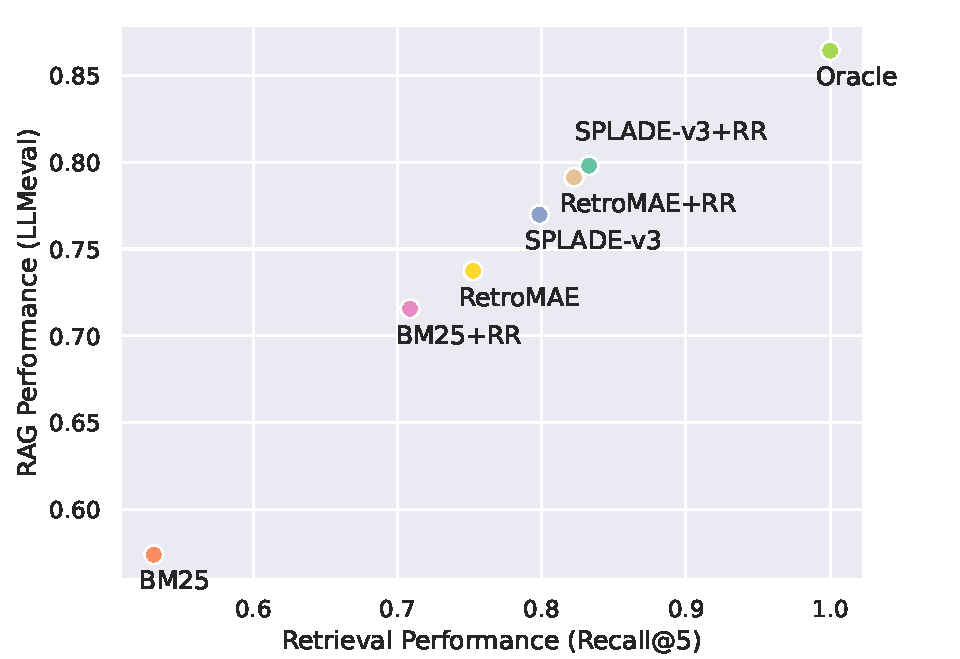
\includegraphics[width=\linewidth]{Figures/RAG_retrievalvsrag.pdf}
		\caption{Impact of retrieval performance on RAG performance for SOLAR-10.7B \cite{kim2024solar} on NQ with different ranking systems. RR means with additional re-ranking using DeBERTa-v3.}
		\label{fig:regencomp01}
	\end{subfigure}
	\hfill
	\begin{subfigure}[b]{0.45\linewidth}
		\centering
		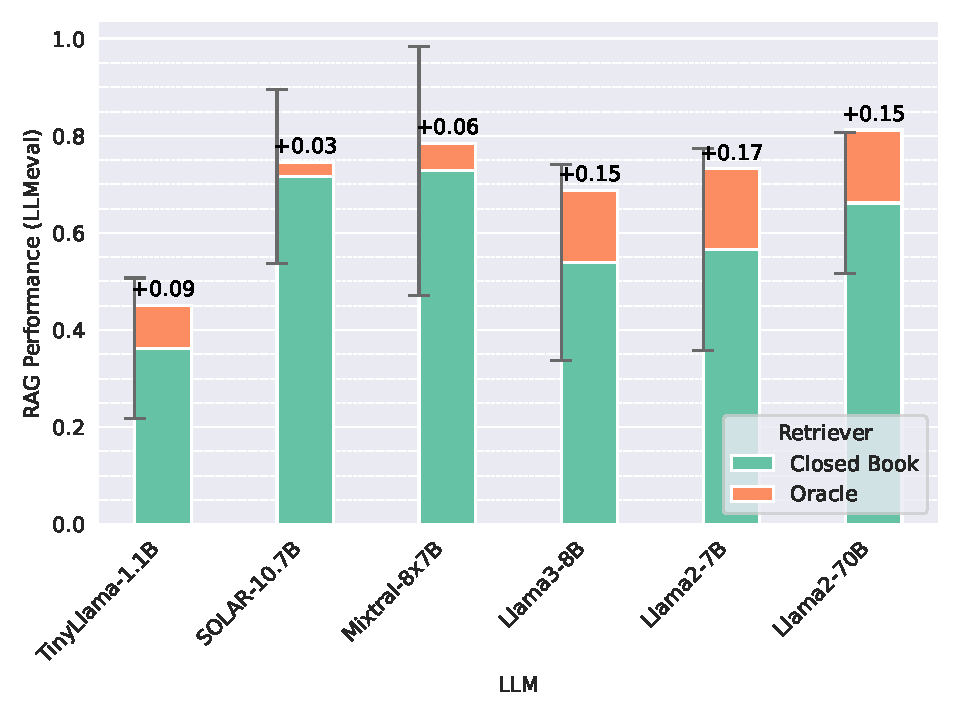
\includegraphics[width=\linewidth]{Figures/RAG_gensize01.pdf}
		\caption{Performance gains w/ and w/o oracle retrieval for LLMs with different sizes. Comparing closed book vs oracle passages averaged over all QA datasets in KILT.}
		\label{fig:regencomp02}
	\end{subfigure}
	
	\begin{subfigure}[b]{\linewidth}
		\centering
		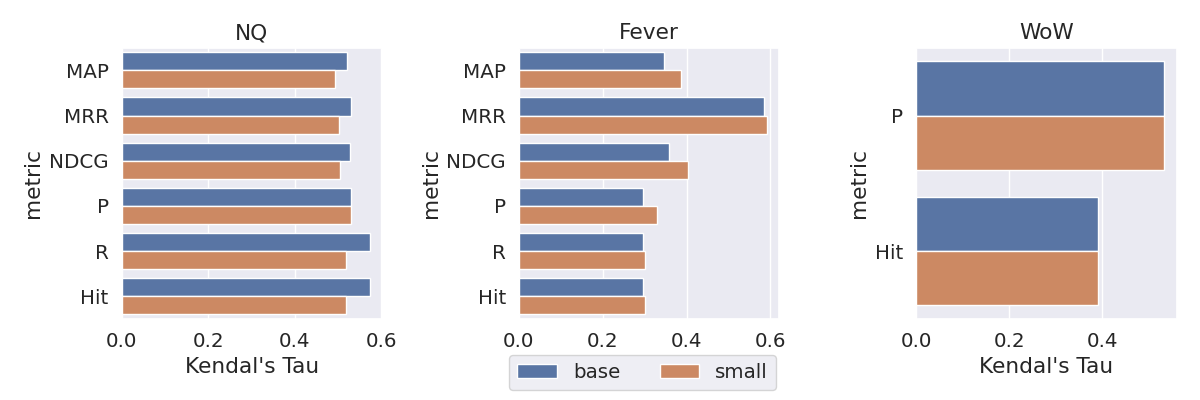
\includegraphics[width=0.9\linewidth]{Figures/RAG_gensize02.png}
		\caption{The correlation between eRAG and the downstream performance of different LLM sizes. In this experiment, T5small (60M parameters) and T5-base (220M parameters) with FiD are used. The documents are retrieved using BM25.}
		\label{fig:regencomp03}
	\end{subfigure}
	
	\caption{Retriever and generator experiment results sourced from eRAG \cite{salemi2024evaluating} and BERGEN \cite{rau2024bergen}.}
	\label{fig:regencomp}
\end{figure}

\subsection{Retriever and Generator}
In RAG, the retriever and generator are central components, each playing a distinct role in the system's overall performance. Table \ref{tab:regencomp} summarizes the retrievers and generators used across the studies discussed in this paper. The table reveals that while a wide range of advanced language models are employed as generators, many systems still rely on traditional retrievers like BM25, valued for their efficiency. This highlights the continued importance of optimizing retrieval methods while balancing computational demands. Interestingly, despite the availability of powerful models such as LLaMA2, GPT-3.5, and GPT-4, these are not widely adopted as generators. Instead, models like T5 remain prevalent, while more foundational retrieval approaches, such as those based on BERT, see limited use. The relative scarcity of IR-focused LLMs in retrievers suggests a promising avenue for future research and development in this domain.

\paragraph{Impact of the Retriever} The results shown in Table \ref{tab:retrievalcomp} highlight the accuracy of GPT-3.5 across different corpora and retrievers on the Mirage benchmark \cite{xiong2024benchmarking}. These findings underscore how retriever performance closely depends on the alignment between training data and the target corpus. For example, in the MEDRAG system, MedCPT—trained specifically on PubMed user logs—significantly improves retrieval performance when accessing the PubMed corpus. This illustrates the benefits of using domain-specific retrievers tailored to specialized datasets. In contrast, general-purpose retrievers like Contriever, which incorporate Wikipedia data during training, excel in retrieving information from Wikipedia, especially for tasks like MMLU-Med and MedQA-US. On the other hand, SPECTER, which focuses more on regularizing pairwise article distances than optimizing query-to-article relevance, underperforms on the MedCorp corpus. The study also explores combining multiple retrievers using Reciprocal Rank Fusion (RRF). However, results show that adding more retrievers does not always lead to better outcomes; for instance, excluding SPECTER in RRF-2 on Wikipedia yields better results than RRF-4, indicating that simply increasing the number of retrievers is not beneficial unless their strengths align with the retrieval task.

Figure \ref{fig:regencomp01} illustrates how eRAG investigates the correlation between LLM performance and retrieval effectiveness on the NQ dataset using three retrievers with different characteristics: BM25 (lexical sparse), RetroMAE (dense) \cite{xiao2022retromae}, and SPLADEv3 (learned sparse) \cite{lassance2024spladev}. The initial retrievals are re-ranked using a DeBERTa-v3 \cite{lassance2022naver} cross-encoder. The analysis demonstrates that as retrieval quality improves, LLM performance increases significantly across various models. Notably, re-ranking with SPLADEv3 and DeBERTa-v3 consistently achieves the best results across datasets and metrics. This underscores the critical role that high-quality retrieval plays in determining overall RAG system effectiveness, suggesting that IR-focused LLMs could be a valuable asset in enhancing generation performance.

\paragraph{Impact of the Generator} The BERGEN study \cite{rau2024bergen} compares the performance of LLMs with gold passages (Oracle) against closed-book settings without retrieval, as shown in Figure \ref{fig:regencomp02}. Surprisingly, the experiments do not reveal a straightforward relationship between model size and the performance gains from retrieval. For instance, smaller models like LLaMA2-7B benefit more from retrieval than larger models like LLaMA2-70B. In fact, LLaMA2-7B with retrieval outperforms LLaMA2-70B in a closed-book setting, suggesting that retrieval augmentation can make smaller models more competitive. Similarly, results from the eRAG experiments in Figure \ref{fig:regencomp03} indicate that varying LLM sizes (e.g., T5-small vs. T5-base) does not significantly affect the correlation between eRAG and downstream performance. These findings highlight that retrieval quality has a more substantial impact on RAG performance than the choice of generator, reinforcing the notion that investing in better retrieval strategies often yields more benefits than relying solely on larger LLMs.